\chapter{Hash Tables}
\chaplabel{hashtables}
\chaplabel{hashing}

Hash tables are an efficient method of storing a small number,
#n#, of integers from a large range $U=\{0,\ldots,2^{#w#}-1\}$.
The term \emph{hash table}
\index{hash table}%
includes a broad range of data structures.  The first part of this
chapter focuses on two of the most common implementations of hash tables:
hashing with chaining and linear probing.

Very often hash tables store types of data that are not integers.
In this case, an integer \emph{hash code}
\index{hash code}%
is associated with each data
item and is used in the hash table.  The second part of this chapter
discusses how such hash codes are generated.

Some of the methods used in this chapter require random choices of
integers in some specific range.  In the code samples, some of these
``random'' integers are hard-coded constants.  These constants were
obtained using random bits generated from atmospheric noise.


\section{#ChainedHashTable#: Hashing with Chaining}
\seclabel{hashtable}

\index{ChainedHashTable@#ChainedHashTable#}%
\index{chaining}%
\index{hashing with chaining}%
A #ChainedHashTable# data structure uses \emph{hashing with chaining} to store
data as an array, #t#, of lists.  An integer, #n#, keeps track of the
total number of items in all lists (see \figref{chainedhashtable}):
\codeimport{ods/ChainedHashTable.t.n}
\begin{figure}
   \begin{center}
     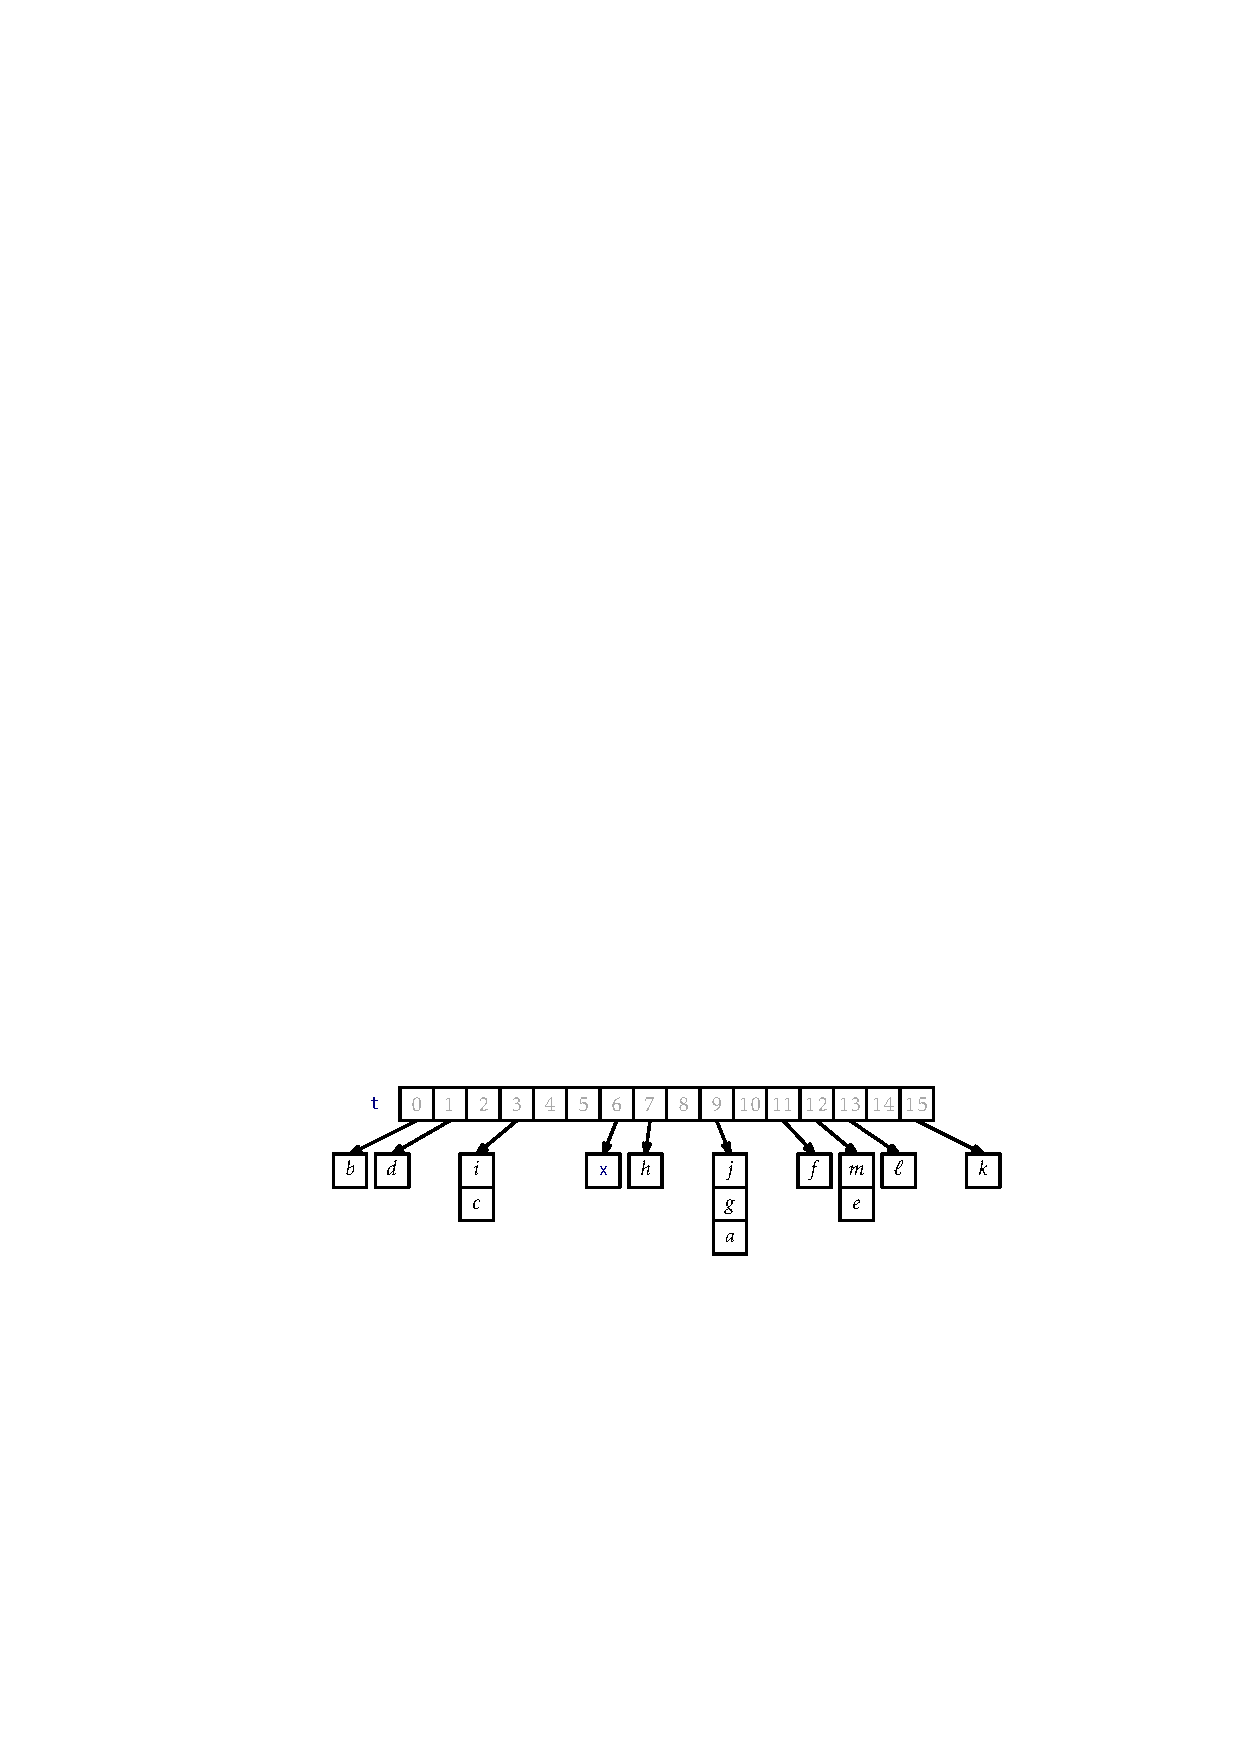
\includegraphics[width=\ScaleIfNeeded]{figs/chainedhashtable}
   \end{center}
   \caption[A ChainedHashTable]{An example of a #ChainedHashTable# with $#n#=14$ and $#t.length#=16$.  In this example $#hash(x)#=6$}
   \figlabel{chainedhashtable}
\end{figure}
\index{hash value}%
\index{hash(x)@#hash(x)#}%
The \emph{hash value} of a data item #x#, denoted #hash(x)# is a value
in the range $\{0,\ldots,#t.length#-1\}$.  All items with hash value #i#
are stored in the list at #t[i]#.  To ensure that lists don't get too
long, we maintain the invariant
\[
    #n# \le #t.length#
\]
so that the average number of elements stored in one of these lists is 
$#n#/#t.length# \le 1$.

To add an element, #x#, to the hash table, we first check if
the length of #t# needs to be increased and, if so, we grow #t#.
With this out of the way we hash #x# to get an integer, #i#, in the
range $\{0,\ldots,#t.length#-1\}$, and we append #x# to the list
#t[i]#:
\codeimport{ods/ChainedHashTable.add(x)}
Growing the table,
if necessary, involves doubling the length of #t# and reinserting
all elements into the new table.  This strategy is exactly the same
as the one used in the implementation of #ArrayStack# and the same
result applies: The cost of growing is only constant when amortized
over a sequence of insertions (see~\lemref{arraystack-amortized} on
page~\pageref{lem:arraystack-amortized}).

Besides growing, the only other work done when adding a new value #x# to a
#ChainedHashTable# involves appending #x# to the list #t[hash(x)]#.  For
any of the list implementations described in Chapters~\ref{chap:arrays}
or \ref{chap:linkedlists}, this takes only constant time.

To remove an element, #x#, from the hash table, we iterate over the list
#t[hash(x)]# until we find #x# so that we can remove it:
\codeimport{ods/ChainedHashTable.remove(x)}
This takes $O(#n#_{#hash(x)#})$ time, where $#n#_{#i#}$ denotes the length
of the list stored at #t[i]#.

Searching for the element #x# in a hash table is similar.  We perform
a linear search on the list #t[hash(x)]#:
\codeimport{ods/ChainedHashTable.find(x)}
Again, this takes time proportional to the length of the list #t[hash(x)]#.

The performance of a hash table depends critically on the choice of the
hash function.  A good hash function will spread the elements evenly
among the #t.length# lists, so that the expected size of the list
#t[hash(x)]# is $O(#n#/#t.length)# = O(1)$.  On the other hand, a bad
hash function will hash all values (including #x#) to the same table
location, in which case the size of the list #t[hash(x)]# will be #n#.
In the next section we describe a good hash function.

\subsection{Multiplicative Hashing}
\seclabel{multihash}

\index{hashing!multiplicative}%
\index{multiplicative hashing}%
Multiplicative hashing is an efficient method of generating hash
values based on modular arithmetic (discussed in \secref{arrayqueue})
and integer division.  It uses the $\ddiv$ operator, which calculates
the integral part of a quotient, while discarding the remainder.
Formally, for any integers $a\ge 0$ and $b\ge 1$, $a\ddiv b = \lfloor
a/b\rfloor$.

In multiplicative hashing, we use a hash table of size $2^{#d#}$ for some
integer #d# (called the \emph{dimension}).  The formula for hashing an
integer $#x#\in\{0,\ldots,2^{#w#}-1\}$ is
\[
    #hash(x)# = ((#z#\cdot#x#) \bmod 2^{#w#}) \ddiv 2^{#w#-#d#} \enspace .
\]
Here, #z# is a randomly chosen \emph{odd} integer in
$\{1,\ldots,2^{#w#}-1\}$.  This hash function can be realized very
efficiently by observing that, by default, operations on integers
are already done modulo $2^{#w#}$ where $#w#$ is the number of bits
in an integer.\footnote{This is true for most programming languages
including C, C\#, C++, and Java. Notable exceptions are Python and
Ruby, in which the result of a fixed-length #w#-bit integer operation
that overflows is upgraded to a variable-length representation.}  (See
\figref{multihashing}.) Furthermore, integer division by $2^{#w#-#d#}$
is equivalent to dropping the rightmost $#w#-#d#$ bits in a binary
representation (which is implemented by shifting the bits right by
$#w#-#d#$ using the \javaonly{#>>>#}\cpponly{#>>#}\pcodeonly{#>>#}
operator).  \notpcode{In this way, the code that implements the above
formula is simpler than the formula itself:}
\codeimport{ods/ChainedHashTable.hash(x)}

\begin{figure}
  \begin{center}
    \resizebox{.98\textwidth}{!}{
    \setlength{\arrayrulewidth}{1pt}
    \begin{tabular}{|lr@{}r|}\hline
    $2^#w#$ (4294967296)&            #1#&#00000000000000000000000000000000# \\
    #z# (4102541685)&                   &#11110100100001111101000101110101# \\
    #x# (42) &                          &#00000000000000000000000000101010# \\
    $#z#\cdot#x#$ &             #101000#&#00011110010010000101110100110010# \\
    $(#z#\cdot#x#)\bmod 2^{#w#}$ &      &#00011110010010000101110100110010# \\
    $((#z#\cdot#x#)\bmod 2^{#w#})\ddiv 2^{#w#-#d#}$ &&
                      \multicolumn{1}{@{}l|}{#00011110#} \\\hline
    \end{tabular}}
    \setlength{\arrayrulewidth}{.4pt}
  \end{center}
  \caption{The operation of the multiplicative hash function with $#w#=32$
    and $#d#=8$.}
  \figlabel{multihashing}
\end{figure}

The following lemma, whose proof is deferred until later in this section,
shows that multiplicative hashing does a good job of avoiding collisions:

\begin{lem}\lemlabel{universal-hashing}
  Let #x# and #y# be any two values in $\{0,\ldots,2^{#w#}-1\}$ with
  $#x#\neq #y#$. Then $\Pr\{#hash(x)#=#hash(y)#\} \le 2/2^{#d#}$.
\end{lem}

With \lemref{universal-hashing}, the performance of #remove(x)#, and
#find(x)# are easy to analyze:

\begin{lem}
  For any data value #x#, the expected length of the list #t[hash(x)]#
  is at most $#n#_{#x#} + 2$, where $#n#_{#x#}$ is the number of
  occurrences of #x# in the hash table.
\end{lem}

\begin{proof}
  Let $S$ be the (multi-)set of elements stored in the hash table that
  are not equal to #x#.  For an element $#y#\in S$, define the indicator
  variable
    \[ I_{#y#} = \left\{\begin{array}{ll}
       1 & \mbox{if $#hash(x)#=#hash(y)#$} \\
       0 & \mbox{otherwise}
       \end{array}\right.
    \]
  and notice that, by \lemref{universal-hashing}, $\E[I_{#y#}] \le
  2/2^{#d#}=2/#t.length#$.  The expected length of the list #t[hash(x)]#
  is given by
  \begin{eqnarray*}
   \E\left[#t[hash(x)].size()#\right] &=& \E\left[#n#_{#x#} + \sum_{#y#\in S} I_{#y#}\right] \\
    &=& #n#_{#x#} + \sum_{#y#\in S} \E [I_{#y#} ] \\
    &\le& #n#_{#x#} + \sum_{#y#\in S} 2/#t.length# \\
    &\le& #n#_{#x#} + \sum_{#y#\in S} 2/#n# \\
    &\le& #n#_{#x#} + (#n#-#n#_{#x#})2/#n# \\
    &\le& #n#_{#x#} + 2 \enspace ,
  \end{eqnarray*}
  as required.
\end{proof}

Now, we want to prove \lemref{universal-hashing}, but first we need a
result from number theory.  In the following proof, we use the notation
$(b_r,\ldots,b_0)_2$ to denote $\sum_{i=0}^r b_i2^i$, where each $b_i$
is a bit, either 0 or 1.  In other words, $(b_r,\ldots,b_0)_2$ is
the integer whose binary representation is given by $b_r,\ldots,b_0$.
We use $\star$ to denote a bit of unknown value.

\begin{lem}\lemlabel{hashing-mapping}
  Let $S$ be the set of odd integers in $\{1,\ldots,2^{#w#}-1\}$; let $q$
  and $i$ be any two elements in $S$.  Then there is exactly one value
  $#z#\in S$ such that $#z#q\bmod 2^{#w#} = i$.
\end{lem}

\begin{proof}
  Since the number of choices for $#z#$ and $i$ is the same, it is
  sufficient to prove that there is \emph{at most} one value $#z#\in S$ that
  satisfies $#z#q\bmod 2^{#w#} = i$.

  Suppose, for the sake of contradiction, that there are two such values
  #z# and #z'#, with $#z#>#z#'$.  Then
  \[
     #z#q\bmod 2^{#w#} = #z#'q \bmod 2^{#w#} = i
  \]
  So
  \[ 
     (#z#-#z#')q\bmod 2^{#w#} = 0 
  \]
  But this means that 
  \begin{equation}
    (#z#-#z#')q = k 2^{#w#} \eqlabel{factors} 
  \end{equation}
  for some integer $k$.  Thinking in terms of binary numbers, we have 
  \[
    (#z#-#z#')q = k\cdot(1,\underbrace{0,\ldots,0}_{#w#})_2 \enspace ,
  \]
  so that the #w# trailing bits in the binary representation of
  $(#z#-#z#')q$ are all 0's.

  Furthermore $k\neq 0$, since $q\neq 0$ and $#z#-#z#'\neq 0$.  Since $q$
  is odd, it has no trailing 0's in its binary representation:
  \[
    q = (\star,\ldots,\star,1)_2 \enspace .
  \]
  Since $|#z#-#z#'| < 2^{#w#}$, $#z#-#z#'$ has fewer than #w# trailing
  0's in its binary representation:
  \[
    #z#-#z#' = (\star,\ldots,\star,1,\underbrace{0,\ldots,0}_{<#w#})_2
      \enspace .
  \]
  Therefore, the product $(#z#-#z#')q$ has fewer than #w# trailing 0's in
  its binary representation:
  \[
   (#z#-#z#')q = (\star,\cdots,\star,1,\underbrace{0,\ldots,0}_{<#w#})_2 
    \enspace .
  \]
  Therefore $(#z#-#z#')q$ cannot satisfy \myeqref{factors}, yielding a
  contradiction and completing the proof.
\end{proof}

The utility of \lemref{hashing-mapping} comes from the following
observation:  If #z# is chosen uniformly at random from $S$, then #zt#
is uniformly distributed over $S$.  In the following proof, it helps
to think of the binary representation of #z#, which consists of $#w#-1$
random bits followed by a 1.

\begin{proof}[Proof of \lemref{universal-hashing}]
  First we note that the condition $#hash(x)#=#hash(y)#$ is equivalent to
  the statement ``the highest-order #d# bits of $#z# #x#\bmod2^{#w#}$
  and the highest-order #d# bits of $#z# #y#\bmod 2^{#w#}$ are the same.''
  A necessary condition of that statement is that the highest-order
  #d# bits in the binary representation of $#z#(#x#-#y#)\bmod 2^{#w#}$
  are either all 0's or all 1's.  That is,
  \begin{equation}
      #z#(#x#-#y#)\bmod 2^{#w#} = 
      (\underbrace{0,\ldots,0}_{#d#},\underbrace{\star,\ldots,\star}_{#w#-#d#})_2 
      \eqlabel{all-zeros}
  \end{equation}
  when $#zx#\bmod 2^{#w#} > #zy#\bmod 2^{#w#}$ or
  \begin{equation}
      #z#(#x#-#y#)\bmod 2^{#w#} = 
      (\underbrace{1,\ldots,1}_{#d#},\underbrace{\star,\ldots,\star}_{#w#-#d#})_2 
       \enspace .
      \eqlabel{all-ones}
  \end{equation}
  when $#zx#\bmod 2^{#w#} < #zy#\bmod 2^{#w#}$.
  Therefore, we only have to bound the probability that 
  $#z#(#x#-#y#)\bmod 2^{#w#}$ looks like \myeqref{all-zeros} or \myeqref{all-ones}.
  
  Let $q$ be the unique odd integer such that $(#x#-#y#)\bmod
  2^{#w#}=q2^r$ for some integer $r\ge 0$. By
  \lemref{hashing-mapping}, the binary representation of $#z#q\bmod
  2^{#w#}$ has $#w#-1$ random bits, followed by a 1:
  \[
   #z#q\bmod 2^{#w#}  = (\underbrace{b_{#w#-1},\ldots,b_{1}}_{#w#-1},1)_2
  \]
  Therefore, the binary representation of $#z#(#x#-#y#)\bmod 2^{#w#}=#z#q2^r\bmod 2^{#w#}$ has
  $#w#-r-1$ random bits, followed by a 1, followed by $r$ 0's:
  \[
  #z#(#x#-#y#)\bmod 2^{#w#}  =
  #z#q2^{r}\bmod 2^{#w#} =
      (\underbrace{b_{#w#-r-1},\ldots,b_{1}}_{#w#-r-1},1,\underbrace{0,0,\ldots,0}_{r})_2
  \]
  We can now finish the proof:  If $r > #w#-#d#$, then the #d#
  higher order bits of $#z#(#x#-#y#)\bmod 2^{#w#}$  contain both 0's
  and 1's, so the probability that $#z#(#x#-#y#)\bmod 2^{#w#}$ looks
  like \myeqref{all-zeros} or \myeqref{all-ones} is 0.  If $#r#=#w#-#d#$,
  then the probability of looking like \myeqref{all-zeros} is 0, but the
  probability of looking like \myeqref{all-ones} is $1/2^{#d#-1}=2/2^{#d#}$
  (since we must have $b_1,\ldots,b_{d-1}=1,\ldots,1$).  If $r < #w#-#d#$,
  then we must have $b_{#w#-r-1},\ldots,b_{#w#-r-#d#}=0,\ldots,0$ or
  $b_{#w#-r-1},\ldots,b_{#w#-r-#d#}=1,\ldots,1$.  The probability of each
  of these cases is $1/2^{#d#}$ and they are mutually exclusive, so the
  probability of either of these cases is $2/2^{#d#}$.  This completes
  the proof.
\end{proof}

\subsection{Summary}

The following theorem summarizes the performance of a #ChainedHashTable#
data structure:

\begin{thm}\thmlabel{hashtable}
  A #ChainedHashTable# implements the #USet# interface.  Ignoring the cost of
  calls to #grow()#, a #ChainedHashTable# supports the operations #add(x)#,
  #remove(x)#, and #find(x)# in $O(1)$ expected time per operation.

  Furthermore, beginning with an empty #ChainedHashTable#, any sequence of
  $m$ #add(x)# and #remove(x)# operations results in a total of $O(m)$
  time spent during all calls to #grow()#.
\end{thm}

\section{#LinearHashTable#: Linear Probing}
\seclabel{linearhashtable}

\index{LinearHashTable@#LinearHashTable#}%
The #ChainedHashTable# data structure uses an array of lists, where the #i#th
list stores all elements #x# such that $#hash(x)#=#i#$.  An alternative,
called \emph{open addressing}
\index{open addressing}%
is to store the elements directly in an
array, #t#, with each array location in #t# storing at most one value.
This approach is taken by the #LinearHashTable# described in this
section.  In some places, this data structure is described as \emph{open
addressing with linear probing}.
\index{linear probing}%

The main idea behind a #LinearHashTable# is that we would, ideally, like
to store the element #x# with hash value #i=hash(x)# in the table location
#t[i]#.  If we cannot do this (because some element is already stored
there) then we try to store it at location $#t#[(#i#+1)\bmod#t.length#]$;
if that's not possible, then we try $#t#[(#i#+2)\bmod#t.length#]$,
and so on, until we find a place for #x#.

There are three types of entries stored in #t#: 
\begin{enumerate}
  \item data values: actual values in the #USet# that we are representing;
  \item #null# values: at array locations where no data has ever been
  stored; and
  \item #del# values: at array locations where data was once stored but that
   has since been deleted.
\end{enumerate}
In addition to the counter, #n#, that keeps track of the number of elements
in the #LinearHashTable#, a counter, #q#, keeps track of the number of
elements of Types~1 and 3.  That is, #q# is equal to #n# plus the number
of #del# values in #t#.  To make this work efficiently, we need
#t# to be considerably larger than #q#, so that there are lots of #null#
values in #t#.  The operations on a #LinearHashTable# therefore maintain
the invariant that $#t.length#\ge 2#q#$.

To summarize, a #LinearHashTable# contains an array, #t#, that stores
data elements, and integers #n# and #q# that keep track of the number of
data elements and non-#null# values of #t#, respectively.  Because many
hash functions only work for table sizes that are a power of 2, we also
keep an integer #d# and maintain the invariant that $#t.length#=2^#d#$.
\codeimport{ods/LinearHashTable.t.n.q.d}

The #find(x)# operation in a #LinearHashTable# is simple.  We start
at array entry #t[i]# where $#i#=#hash(x)#$ and search entries #t[i]#,
$#t#[(#i#+1)\bmod #t.length#]$, $#t#[(#i#+2)\bmod #t.length#]$, and so on,
until we find an index #i'# such that, either, #t[i']=x#, or #t[i']=null#.
In the former case we return #t[i']#. In the latter case, we conclude
that #x# is not contained in the hash table and return #null#.
\codeimport{ods/LinearHashTable.find(x)}

The #add(x)# operation is also fairly easy to implement. After checking
that #x# is not already stored in the table (using #find(x)#), we search
#t[i]#, $#t#[(#i#+1)\bmod #t.length#]$, $#t#[(#i#+2)\bmod #t.length#]$,
and so on, until we find a #null# or #del# and store #x# at that location,
increment #n#, and #q#, if appropriate.
\codeimport{ods/LinearHashTable.add(x)}

By now, the implementation of the #remove(x)# operation should be obvious.
We search #t[i]#, $#t#[(#i#+1)\bmod #t.length#]$, $#t#[(#i#+2)\bmod
#t.length#]$, and so on until we find an index #i'# such that #t[i']=x#
or #t[i']=null#.  In the former case, we set #t[i']=del# and return
#true#.  In the latter case we conclude that #x# was not stored in the
table (and therefore cannot be deleted) and return #false#.
\codeimport{ods/LinearHashTable.remove(x)}

The correctness of the #find(x)#, #add(x)#, and #remove(x)# methods is
easy to verify, though it relies on the use of #del# values.  Notice
that none of these operations ever sets a non-#null# entry to #null#.
Therefore, when we reach an index #i'# such that #t[i']=null#, this is
a proof that the element, #x#, that we are searching for is not stored
in the table; #t[i']# has always been #null#, so there is no reason that
a previous #add(x)# operation would have proceeded beyond index #i'#.

The #resize()# method is called by #add(x)# when the number of non-#null#
entries exceeds $#t.length#/2$ or by #remove(x)# when the number of
data entries is less than #t.length/8#.  The #resize()# method works
like the #resize()# methods in other array-based data structures.
We find the smallest non-negative integer #d# such that $2^{#d#}
\ge 3#n#$.  We reallocate the array #t# so that it has size $2^{#d#}$,
and then we insert all the elements in the old version of #t# into the
newly-resized copy of #t#.  While doing this, we reset #q# equal to #n#
since the newly-allocated #t# contains no #del# values.
\codeimport{ods/LinearHashTable.resize()}

\subsection{Analysis of Linear Probing}

Notice that each operation, #add(x)#, #remove(x)#, or #find(x)#, finishes
as soon as (or before) it discovers the first #null# entry in #t#.
The intuition behind the analysis of linear probing is that, since at
least half the elements in #t# are equal to #null#, an operation should
not take long to complete because it will very quickly come across a
#null# entry.  We shouldn't rely too heavily on this intuition, though,
because it would lead us to (the incorrect) conclusion that the expected
number of locations in #t# examined by an operation is at most 2.

For the rest of this section, we will assume that all hash values are
independently and uniformly distributed in $\{0,\ldots,#t.length#-1\}$.
This is not a realistic assumption, but it will make it possible for
us to analyze linear probing.  Later in this section we will describe a
method, called tabulation hashing, that produces a hash function that is
``good enough'' for linear probing.  We will also assume that all indices
into the positions of #t# are taken modulo #t.length#, so that #t[i]#
is really a shorthand for $#t#[#i#\bmod#t.length#]$.

\index{run}%
We say that a \emph{run of length $k$ that starts at #i#} occurs when all
the table entries $#t[i]#, #t[i+1]#,\ldots,#t#[#i#+k-1]$ are non-#null#
and $#t#[#i#-1]=#t#[#i#+k]=#null#$.  The number of non-#null# elements of
#t# is exactly #q# and the #add(x)# method ensures that, at all times,
$#q#\le#t.length#/2$.  There are #q# elements $#x#_1,\ldots,#x#_{#q#}$
that have been inserted into #t# since the last #resize()# operation.
By our assumption, each of these has a hash value, $#hash#(#x#_j)$,
that is uniform and independent of the rest.  With this setup, we can
prove the main lemma required to analyze linear probing.

\begin{lem}\lemlabel{linear-probing}
Fix a value $#i#\in\{0,\ldots,#t.length#-1\}$.  Then the probability that
a run of length $k$ starts at #i# is $O(c^k)$ for some constant $0<c<1$.
\end{lem}

\begin{proof}
If a run of length $k$ starts at #i#, then there are exactly $k$
elements $#x#_j$ such that $#hash#(#x#_j)\in\{#i#,\ldots,#i#+k-1\}$.
The probability that this occurs is exactly
\[
  p_k  = \binom{#q#}{k}\left(\frac{k}{#t.length#}\right)^k\left(\frac{#t.length#-k}{#t.length#}\right)^{#q#-k} \enspace ,
\]
since, for each choice of $k$ elements, these $k$ elements must hash to
one of the $k$ locations and the remaining $#q#-k$ elements must hash to
the other $#t.length#-k$ table locations.\footnote{Note that $p_k$ is greater
than the probability that a run of length $k$ starts at #i#, since the definition of $p_k$ does not include the requirement $#t#[#i#-1]=#t#[#i#+k]=#null#$.}

In the following derivation we will cheat a little and replace $r!$ with
$(r/e)^r$. Stirling's Approximation (\secref{factorials}) shows that this
is only a factor of $O(\sqrt{r})$ from the truth.  This is just done to
make the derivation simpler; \excref{linear-probing} asks the reader to
redo the calculation more rigorously using Stirling's Approximation in
its entirety.

The value of $p_k$ is maximized when #t.length# is minimum, and the data
structure maintains the invariant that $#t.length# \ge 2#q#$, so
\begin{align*}
   p_k & \le \binom{#q#}{k}\left(\frac{k}{2#q#}\right)^k\left(\frac{2#q#-k}{2#q#}\right)^{#q#-k} \\
  & = \left(\frac{#q#!}{(#q#-k)!k!}\right)\left(\frac{k}{2#q#}\right)^k\left(\frac{2#q#-k}{2#q#}\right)^{#q#-k} \\
  & \approx \left(\frac{#q#^{#q#}}{(#q#-k)^{#q#-k}k^k}\right)\left(\frac{k}{2#q#}\right)^k\left(\frac{2#q#-k}{2#q#}\right)^{#q#-k} && \text{[Stirling's approximation]} \\
  & = \left(\frac{#q#^{k}#q#^{#q#-k}}{(#q#-k)^{#q#-k}k^k}\right)\left(\frac{k}{2#q#}\right)^k\left(\frac{2#q#-k}{2#q#}\right)^{#q#-k} \\
 & = \left(\frac{#q#k}{2#q#k}\right)^k
     \left(\frac{#q#(2#q#-k)}{2#q#(#q#-k)}\right)^{#q#-k} \\
 & = \left(\frac{1}{2}\right)^k
     \left(\frac{(2#q#-k)}{2(#q#-k)}\right)^{#q#-k} \\
 & = \left(\frac{1}{2}\right)^k
     \left(1+\frac{k}{2(#q#-k)}\right)^{#q#-k} \\
 & \le \left(\frac{\sqrt{e}}{2}\right)^k \enspace .
\end{align*}
(In the last step, we use the inequality $(1+1/x)^x \le e$, which holds
for all $x>0$.)  Since $\sqrt{e}/{2}< 0.824360636 < 1$, this completes
the proof.
\end{proof}

Using \lemref{linear-probing} to prove upper-bounds on the expected
running time of #find(x)#, #add(x)#, and #remove(x)# is now fairly
straightforward.  Consider the simplest case, where we execute
#find(x)# for some value #x# that has never been stored in the
#LinearHashTable#.  In this case, $#i#=#hash(x)#$ is a random value in
$\{0,\ldots,#t.length#-1\}$ independent of the contents of #t#.  If #i#
is part of a run of length $k$, then the time it takes to execute the
#find(x)# operation is at most $O(1+k)$.  Thus, the expected running time
can be upper-bounded by
\[
  O\left(1 + \left(\frac{1}{#t.length#}\right)\sum_{i=1}^{#t.length#}\sum_{k=0}^{\infty} k\Pr\{\text{#i# is part of a run of length $k$}\}\right) \enspace .
\]
Note that each run of length $k$ contributes to the inner sum $k$ times for a total contribution of $k^2$,  so the above sum can be rewritten as
\begin{align*}
  & { } O\left(1 + \left(\frac{1}{#t.length#}\right)\sum_{i=1}^{#t.length#}\sum_{k=0}^{\infty} k^2\Pr\{\mbox{#i# starts a run of length $k$}\}\right) \\
  & \le O\left(1 + \left(\frac{1}{#t.length#}\right)\sum_{i=1}^{#t.length#}\sum_{k=0}^{\infty} k^2p_k\right) \\
  & = O\left(1 + \sum_{k=0}^{\infty} k^2p_k\right) \\
  & = O\left(1 + \sum_{k=0}^{\infty} k^2\cdot O(c^k)\right) \\
  & = O(1) \enspace .
\end{align*}
The last step in this derivation comes from the fact that
$\sum_{k=0}^{\infty} k^2\cdot O(c^k)$ is an exponentially decreasing
series.\footnote{In the terminology of many calculus texts, this sum
passes the ratio test:  There exists a positive integer $k_0$ such
that, for all $k\ge k_0$, $\frac{(k+1)^2c^{k+1}}{k^2c^k} < 1$.}
Therefore, we conclude that the expected running time of the #find(x)# operation
for a value #x# that is not contained in a #LinearHashTable# is $O(1)$.

If we ignore the cost of the #resize()# operation, then the above
analysis gives us all we need to analyze the cost of operations on a
#LinearHashTable#.

First of all, the analysis of #find(x)# given above applies to the
#add(x)# operation when #x# is not contained in the table.  To analyze
the #find(x)# operation when #x# is contained in the table, we need only
note that this is the same as the cost of the #add(x)# operation that
previously added #x# to the table.  Finally, the cost of a #remove(x)#
operation is the same as the cost of a #find(x)# operation.

In summary, if we ignore the cost of calls to #resize()#, all operations
on a #LinearHashTable# run in $O(1)$ expected time.  Accounting for the
cost of resize can be done using the same type of amortized analysis
performed for the #ArrayStack# data structure in \secref{arraystack}.

\subsection{Summary}

The following theorem summarizes the performance of the #LinearHashTable#
data structure:

\begin{thm}\thmlabel{linear-probing}
  A #LinearHashTable# implements the #USet# interface.  Ignoring the
  cost of calls to #resize()#, a #LinearHashTable# supports the operations
  #add(x)#, #remove(x)#, and #find(x)# in $O(1)$ expected time per
  operation.  

  Furthermore, beginning with an empty #LinearHashTable#, any
  sequence of $m$ #add(x)# and #remove(x)# operations results in a total
  of $O(m)$ time spent during all calls to #resize()#.
\end{thm}

\subsection{Tabulation Hashing}
\seclabel{tabulation}

\index{tabulation hashing}%
While analyzing the #LinearHashTable# structure, we made a very strong
assumption:  That for any set of elements, $\{#x#_1,\ldots,#x#_#n#\}$,
the hash values $#hash#($x$_1),\ldots,#hash#(#x#_#n#)$ are independently and
uniformly distributed over the set $\{0,\ldots,#t.length#-1\}$.  One way to
achieve this is to store a giant array, #tab#, of length $2^{#w#}$,
where each entry is a random #w#-bit integer, independent of all the
other entries.  In this way, we could implement #hash(x)# by extracting
a #d#-bit integer from #tab[x.hashCode()]#:
\codeimport{ods/LinearHashTable.idealHash(x)}
\pcodeonly{Here, #>>#, is the \emph{bitwise right shift} operator, so
#x.hashCode() >> w-d# extracts the #d# most significant bits of #x#'s #w#-bit hash code.}

Unfortunately, storing an array of size $2^{#w#}$ is prohibitive in terms
of memory usage.  The approach used by \emph{tabulation hashing} is to,
instead, treat #w#-bit integers as being comprised of $#w#/#r#$
integers, each having only $#r#$ bits.  In this way, tabulation hashing
only needs $#w#/#r#$ arrays each of length $2^{#r#}$.  All the entries
in these arrays are independent random #w#-bit integers.  To obtain the value
of #hash(x)# we split #x.hashCode()# up into $#w#/#r#$ #r#-bit integers
and use these as indices into these arrays.  We then combine all these
values with the bitwise exclusive-or operator to obtain #hash(x)#.
The following code shows how this works when $#w#=32$ and $#r#=4$:
\codeimport{ods/LinearHashTable.hash(x)}
In this case, #tab# is a two-dimensional array with four columns and
$2^{32/4}=256$ rows.
\pcodeonly{
Quantities like #0xff#, used above, are \emph{hexadecimal numbers}
\index{hexadecimal numbers}%
whose digits have 16 possible values 0--9, which have their usual
meaning and a--f, which denote 10--15.  The number $#0xff#=15\cdot 16 + 15 = 255$.
The #&# symbol is the \emph{bitwise and} operator, so
code like #h >> 8 & 0xff# extracts bits with index 8 through 15 of #h#.}

One can easily verify that, for any #x#, #hash(x)# is uniformly
distributed over $\{0,\ldots,2^{#d#}-1\}$.  With a little work, one
can even verify that any pair of values have independent hash values.
This implies tabulation hashing could be used in place of multiplicative
hashing for the #ChainedHashTable# implementation.

However, it is not true that any set of #n# distinct values gives a set
of #n# independent hash values.  Nevertheless, when tabulation hashing is
used, the bound of \thmref{linear-probing} still holds.  References for
this are provided at the end of this chapter.

\section{Hash Codes}

\index{hash code}%
The hash tables discussed in the previous section are used to associate
data with integer keys consisting of #w# bits.  In many cases, we
have keys that are not integers.  They may be strings, objects, arrays,
or other compound structures.  To use hash tables for these types of data,
we must map these data types to #w#-bit hash codes.  Hash code mappings should
have the following properties:

\begin{enumerate}
  \item If #x# and #y# are equal, then #x.hashCode()# and #y.hashCode()#
  are equal.

  \item If #x# and #y# are not equal, then the probability that
  $#x.hashCode()#=#y.hashCode()#$ should be small (close to
  $1/2^{#w#}$).
\end{enumerate}

The first property ensures that if we store #x# in a hash table and later
look up a value #y# equal to #x#, then we will find #x#---as we should.
The second property minimizes the loss from converting our objects
to integers.  It ensures that unequal objects usually have different
hash codes and so are likely to be stored at different locations in
our hash table.

\subsection{Hash Codes for Primitive Data Types}

\index{hash code!for primitive data}%
Small primitive data types like #char#, #byte#, #int#, and #float# are
usually easy to find hash codes for.  These data types always have a
binary representation and this binary representation usually consists of
#w# or fewer bits. \javaonly{(For example, in Java, #byte# is an 8-bit
type and #float# is a 32-bit type.)}\cpponly{(For example, in C++ #char#
is typically an 8-bit type and #float# is a 32-bit type.)} In these
cases, we just treat these bits as the representation of an integer in
the range $\{0,\ldots,2^#w#-1\}$.  If two values are different, they get
different hash codes.  If they are the same, they get the same hash code.

A few primitive data types are made up of more than #w# bits, usually
$c#w#$ bits for some constant integer $c$. (Java's #long# and #double#
types are examples of this with $c=2$.)  These data types can be treated
as compound objects made of $c$ parts, as described in the next section.

\subsection{Hash Codes for Compound Objects}
\seclabel{stringhash}

\index{hash code!for compound objects}%
For a compound object, we want to create a hash code by combining the
individual hash codes of the object's constituent parts.  This is not
as easy as it sounds.  Although one can find many hacks for this (for
example, combining the hash codes with bitwise exclusive-or operations),
many of these hacks turn out to be easy to foil (see Exercises~\ref{exc:hash-hack-first}--\ref{exc:hash-hack-last}).
However, if one is willing to do arithmetic with $2#w#$ bits of
precision, then there are simple and robust methods available.
Suppose we have an object made up of several parts
$P_0,\ldots,P_{r-1}$ whose hash codes are $#x#_0,\ldots,#x#_{r-1}$.
Then we can choose mutually independent random #w#-bit integers
$#z#_0,\ldots,#z#_{r-1}$ and a random $2#w#$-bit odd integer #z# and
compute a hash code for our object with
\[
   h(#x#_0,\ldots,#x#_{r-1}) =  
   \left(\left(#z#\sum_{i=0}^{r-1} #z#_i #x#_i\right)\bmod 2^{2#w#}\right)
   \ddiv 2^{#w#} \enspace .
\]
Note that this hash code has a final step (multiplying by #z# and
dividing by $2^{#w#}$) that uses the multiplicative hash function
from \secref{multihash} to take the $2#w#$-bit intermediate result and
reduce it to a #w#-bit final result.  Here is an example of this method applied to a simple compound object with three parts #x0#, #x1#, and #x2#:
\javaimport{junk/Point3D.x0.hashCode()}
\cppimport{ods/Point3D.hashCode()}
\pcodeimport{ods/Point3d.hashCode()}
The following theorem shows that, in addition to being straightforward to implement, this method is provably good:

\begin{thm}\thmlabel{multihash}
Let $#x#_0,\ldots,#x#_{r-1}$ and $#y#_0,\ldots,#y#_{r-1}$ each be sequences of #w# bit integers in $\{0,\ldots,2^{#w#}-1\}$ and assume $#x#_i \neq #y#_i$ for at least one index $i\in\{0,\ldots,r-1\}$. Then 
\[
   \Pr\{ h(#x#_0,\ldots,#x#_{r-1}) =  h(#y#_0,\ldots,#y#_{r-1}) \} 
        \le 3/2^{#w#} \enspace .  
\] 
\end{thm}

\begin{proof}
  We will first ignore the final multiplicative hashing step and see how
  that step contributes later.  Define:
  \[
    h'(#x#_0,\ldots,#x#_{r-1}) =  
       \left(\sum_{j=0}^{r-1} #z#_j #x#_j\right)\bmod 2^{2#w#} \enspace .
  \]
  Suppose that $h'(#x#_0,\ldots,#x#_{r-1}) =  h'(#y#_0,\ldots,#y#_{r-1})$.
  We can rewrite this as:
  \begin{equation}  \eqlabel{bighash-x}
      #z#_i(#x#_i-#y#_i) \bmod 2^{2#w#} = t
  \end{equation}
  where 
  \[
     t = \left(\sum_{j=0}^{i-1} #z#_j(#y#_j-#x#_j) + \sum_{j=i+1}^{r-1} #z#_j(#y#_j-#x#_j)\right) \bmod 2^{2#w#}
  \]
  If we assume, without loss of generality that $#x#_i> #y#_i$, then
  \myeqref{bighash-x} becomes
  \begin{equation}
      #z#_i(#x#_i-#y#_i) = t \eqlabel{bighash-xx} \enspace ,
  \end{equation}
  since each of $#z#_i$ and $(#x#_i-#y#_i)$ is at most $2^{#w#}-1$, so
  their product is at most $2^{2#w#}-2^{#w#+1}+1 < 2^{2#w#}-1$.
  By assumption, $#x#_i-#y#_i\neq 0$, so \myeqref{bighash-xx} has at most one
  solution in $#z#_i$.  Therefore, since $#z#_i$ and $t$ are
  independent ($#z#_0,\ldots,#z#_{r-1}$ are mutually independent), the
  probability that we select $#z#_i$
  so that $h'(#x#_0,\ldots,#x#_{r-1})=h'(#y#_0,\ldots,#y#_{r-1})$ is at most
  $1/2^{#w#}$.

  The final step of the hash function is to apply multiplicative hashing
  to reduce our $2#w#$-bit intermediate result $h'(#x#_0,\ldots,#x#_{r-1})$ to
  a #w#-bit final result $h(#x#_0,\ldots,#x#_{r-1})$.  By \thmref{multihash},
  if $h'(#x#_0,\ldots,#x#_{r-1})\neq h'(#y#_0,\ldots,#y#_{r-1})$, then
  $\Pr\{h(#x#_0,\ldots,#x#_{r-1}) = h(#y#_0,\ldots,#y#_{r-1})\} \le 2/2^{#w#}$.

  To summarize, 
  \begin{align*}
    & \Pr\left\{\begin{array}{l}
          h(#x#_0,\ldots,#x#_{r-1}) \\
          \quad = h(#y#_0,\ldots,#y#_{r-1})\end{array}\right\} \\
      &= \Pr\left\{\begin{array}{ll}
            \mbox{$h'(#x#_0,\ldots,#x#_{r-1}) = h'(#y#_0,\ldots,#y#_{r-1})$ or} \\
            \mbox{$h'(#x#_0,\ldots,#x#_{r-1}) \neq h'(#y#_0,\ldots,#y#_{r-1})$} \\
                 \quad  \mbox{and
$#z#h'(#x#_0,\ldots,#x#_{r-1})\ddiv2^{#w#} = #z# h'(#y#_0,\ldots,#y#_{r-1})\ddiv 2^{#w#}$}
          \end{array}\right\} \\
      &\le 1/2^{#w#} + 2/2^{#w#} = 3/2^{#w#} \enspace . \qedhere
  \end{align*}
\end{proof}


\index{hash code!for strings}%
\index{hash code!for arrays}%
\subsection{Hash Codes for Arrays and Strings}
\seclabel{polyhash}

The method from the previous section works well for objects that have a
fixed, constant, number of components.  However, it breaks down when we
want to use it with objects that have a variable number of components,
since it requires a random #w#-bit integer $#z#_i$ for each component.
We could use a pseudorandom sequence to generate as many $#z#_i$'s as we
need, but then the $#z#_i$'s are not mutually independent, and it becomes
difficult to prove that the pseudorandom numbers don't interact badly
with the hash function we are using.  In particular, the values of $t$
and $#z#_i$ in the proof of \thmref{multihash} are no longer independent.

\index{prime field}%
A more rigorous approach is to base our hash codes on polynomials over
prime fields;  these are just regular polynomials that are evaluated
modulo some prime number, #p#. This method is based on the following
theorem, which says that polynomials over prime fields behave pretty-much
like usual polynomials:

\begin{thm}\thmlabel{prime-polynomial}
 Let $#p#$ be a prime number, and let $f(#z#) = #x#_0#z#^0 + #x#_1#z#^1 +
 \cdots + #x#_{r-1}#z#^{r-1}$ be a non-trivial polynomial with coefficients
 $#x#_i\in\{0,\ldots,#p#-1\}$. Then the equation $f(#z#)\bmod #p# = 0$
 has at most $r-1$ solutions for $#z#\in\{0,\ldots,p-1\}$.
\end{thm}

To use \thmref{prime-polynomial}, we hash a sequence of integers
$#x#_0,\ldots,#x#_{r-1}$ with each $#x#_i\in \{0,\ldots,#p#-2\}$ using
a random integer $#z#\in\{0,\ldots,#p#-1\}$ via the formula
\[
   h(#x#_0,\ldots,#x#_{r-1}) 
    = \left(#x#_0#z#^0+\cdots+#x#_{r-1}#z#^{r-1}+(#p#-1)#z#^r \right)\bmod #p# \enspace .
\]

Note the extra $(#p#-1)#z#^r$ term at the end of the formula.  It helps
to think of $(#p#-1)$ as the last element, $#x#_r$, in the sequence
$#x#_0,\ldots,#x#_{r}$.  Note that this element differs from every other
element in the sequence (each of which is in the set $\{0,\ldots,#p#-2\}$).
We can think of $#p#-1$ as an end-of-sequence marker.

The following theorem, which considers the case of two sequences of
the same length, shows that this hash function gives a good return for
the small amount of randomization needed to choose #z#:

\begin{thm}\thmlabel{stringhash-eqlen}
  Let $#p#>2^{#w#}+1$ be a prime, let $#x#_0,\ldots,#x#_{r-1}$ and
  $#y#_0,\ldots,#y#_{r-1}$ each be sequences of #w#-bit integers in
  $\{0,\ldots,2^{#w#}-1\}$, and assume $#x#_i \neq #y#_i$ for at least
  one index $i\in\{0,\ldots,r-1\}$. Then
  \[
     \Pr\{ h(#x#_0,\ldots,#x#_{r-1}) =  h(#y#_0,\ldots,#y#_{r-1}) \} 
          \le (r-1)/#p# \enspace .
  \] 
\end{thm}

\begin{proof}
  The equation $h(#x#_0,\ldots,#x#_{r-1}) =  h(#y#_0,\ldots,#y#_{r-1})$
  can be rewritten as
  \begin{equation}  \eqlabel{strhash-eqlen}
    \left(
       (#x#_0-#y#_0)#z#^0+\cdots+(#x#_{r-1}-#y#_{r-1})#z#^{r-1} 
    \right)\bmod #p# = 0.
  \end{equation}
  Since $#x#_#i#\neq #y#_#i#$, this polynomial is non-trivial.  Therefore,
  by \thmref{prime-polynomial}, it has at most $r-1$ solutions in #z#.
  The probability that we pick #z# to be one of these solutions is therefore
  at most $(r-1)/#p#$.
\end{proof}

Note that this hash function also deals with the case in which two
sequences have different lengths, even when one of the sequences is a
prefix of the other. This is because this function effectively hashes
the infinite sequence
\[
  #x#_0,\ldots,#x#_{r-1}, #p#-1,0,0,\ldots \enspace .
\]
This guarantees that if we have two sequences of length $r$ and $r'$
with $r > r'$, then these two sequences differ at index $i=r$.  In
this case, \myeqref{strhash-eqlen} becomes
\[
  \left(
     \sum_{i=0}^{i=r'-1}(#x#_i-#y#_i)#z#^i + (#x#_{r'} - #p# + 1)#z#^{r'}
     +\sum_{i=r'+1}^{i=r-1}#x#_i#z#^i + (#p#-1)#z#^{r}
  \right)\bmod #p# = 0 \enspace ,
\]
which, by \thmref{prime-polynomial}, has at most $r$ solutions in $#z#$.
This combined with \thmref{stringhash-eqlen} suffice to prove the
following more general theorem:

\begin{thm}\thmlabel{stringhash}
  Let $#p#>2^{#w#}+1$ be a prime, let $#x#_0,\ldots,#x#_{r-1}$ and
  $#y#_0,\ldots,#y#_{r'-1}$ be distinct sequences of #w#-bit integers in
  $\{0,\ldots,2^{#w#}-1\}$. Then
  \[
     \Pr\{ h(#x#_0,\ldots,#x#_{r-1}) =  h(#y#_0,\ldots,#y#_{r-1}) \} 
          \le \max\{r,r'\}/#p#  \enspace .  
  \] 
\end{thm}

The following example code shows how this hash function is applied to
an object that contains an array, #x#, of values:
\javaimport{junk/GeomVector.hashCode()}
\cppimport{ods/GeomVector.hashCode()}
\pcodeimport{ods/GeomVector.hashCode()}

The preceding code sacrifices some collision probability for implementation
convenience.  In particular, it applies the multiplicative hash function
from \secref{multihash}, with $#d#=31$ to reduce #x[i].hashCode()# to a
31-bit value.  This is so that the additions and multiplications that are
done modulo the prime $#p#=2^{32}-5$ can be carried out using unsigned
63-bit arithmetic.  Thus the probability of two different sequences,
the longer of which has length $r$, having the same hash code is at most
\[
    2/2^{31} + r/(2^{32}-5)
\]
rather than the $r/(2^{32}-5)$ specified in \thmref{stringhash}.

\section{Discussion and Exercises}

Hash tables and hash codes represent an enormous and active field
of research that is just touched upon in this chapter.  The online
Bibliography on Hashing \cite{hashing}
\index{Bibliography on Hashing}%
contains nearly 2000 entries.

A variety of different hash table implementations exist. The one
described in \secref{hashtable} is known as \emph{hashing with chaining}
\index{hashing with chaining}%
(each array entry contains a chain (#List#) of elements).  Hashing with
chaining dates back to an internal IBM memorandum authored by H. P. Luhn
and dated January 1953. This memorandum also seems to be one of the
earliest references to linked lists.

\index{open addressing}%
An alternative to hashing with chaining is that used by \emph{open
addressing} schemes, where all data is stored directly in an
array.  These schemes include the #LinearHashTable# structure of
\secref{linearhashtable}. This idea was also proposed, independently, by
a group at IBM in the 1950s.  Open addressing schemes must deal with the
problem of \emph{collision resolution}: 
\index{collision resolution}%
the case where two values hash
to the same array location.  Different strategies exist for collision
resolution; these provide different performance guarantees and often
require more sophisticated hash functions than the ones described here.

Yet another category of hash table implementations are the so-called
\emph{perfect hashing} methods.
\index{perfect hashing}%
These are methods in which #find(x)#
operations take $O(1)$ time in the worst-case.  For static data sets,
this can be accomplished by finding \emph{perfect hash functions}
\index{perfect hash function}%
\index{hash function!perfect}%
for
the data; these are functions that map each piece of data to a unique
array location.  For data that changes over time, perfect hashing
methods include \emph{FKS two-level hash tables}
\index{two-level hash table}%
\index{hash table!two-level}%
\cite{fks84,dkkmrt94}
and \emph{cuckoo hashing} \cite{pr04}.
\index{cuckoo hashing}%
\index{hash table!cuckoo}%

The hash functions presented in this chapter are probably among the most
practical methods currently known that can be proven to work well for any
set of data.  Other provably good methods date back to the pioneering work
of Carter and Wegman who introduced the notion of \emph{universal hashing}
\index{universal hashing}%
\index{hashing!universal}%
and described several hash functions for different scenarios \cite{cw79}.
Tabulation hashing, described in \secref{tabulation}, is due to Carter
and Wegman \cite{cw79}, but its analysis, when applied to linear probing
(and several other hash table schemes) is due to P\v{a}tra\c{s}cu and
Thorup \cite{pt12}.

The idea of \emph{multiplicative hashing}
\index{multiplicative hashing}%
\index{hashing!multiplicative}%
is very old and seems to be
part of the hashing folklore \cite[Section~6.4]{k97v3}.  However, the
idea of choosing the multiplier #z# to be a random \emph{odd} number,
and the analysis in \secref{multihash} is due to Dietzfelbinger \etal\
\cite{dhkp97}.  This version of multiplicative hashing is one of the
simplest, but its collision probability of $2/2^{#d#}$ is a factor of two
larger than what one could expect with a random function from $2^{#w#}\to
2^{#d#}$.  The \emph{multiply-add hashing}
\index{hashing!multiply-add}%
\index{multiply-add hashing}%
method uses the function
\[
   h(#x#) = ((#z##x# + b) \bmod 2^{#2w#}) \ddiv 2^{#2w#-#d#}
\]
where #z# and #b# are each randomly chosen from $\{0,\ldots,2^{#2w#}-1\}$.
Multiply-add hashing has a collision probability of only $1/2^{#d#}$
\cite{d96}, but requires $2#w#$-bit precision arithmetic.

There are a number of methods of obtaining hash codes from fixed-length
sequences of #w#-bit integers.  One particularly fast method
\cite{bhkkr99} is the function
\[\begin{array}{l}
  h(#x#_0,\ldots,#x#_{r-1}) \\
   \quad = \left(\sum_{i=0}^{r/2-1} ((#x#_{2i}+#a#_{2i})\bmod 2^{#w#})((#x#_{2i+1}+#a#_{2i+1})\bmod 2^{#w#})\right) \bmod 2^{2#w#}
\end{array}
\]
where $r$ is even and $#a#_0,\ldots,#a#_{r-1}$ are randomly chosen from
$\{0,\ldots,2^{#w#}\}$. This yields a $2#w#$-bit hash code that has
collision probability $1/2^{#w#}$.  This can be reduced to a #w#-bit hash
code using multiplicative (or multiply-add) hashing. This method is fast
because it requires only $r/2$ $2#w#$-bit multiplications whereas the
method described in \secref{stringhash} requires $r$ multiplications.
(The $\bmod$ operations occur implicitly by using #w# and $2#w#$-bit
arithmetic for the additions and multiplications, respectively.)

The method from \secref{polyhash} of using polynomials over prime fields
to hash variable-length arrays and strings is due to Dietzfelbinger \etal\
\cite{dgmp92}.  Due to its use of the $\bmod$ operator which relies
on a costly machine instruction, it is, unfortunately, not very fast.
Some variants of this method choose the prime #p# to be one of the form
$2^{#w#}-1$, in which case the $\bmod$ operator can be replaced with
addition (#+#) and bitwise-and (#&#) operations \cite[Section~3.6]{k97v2}.
Another option is to apply one of the fast methods for fixed-length
strings to blocks of length $c$ for some constant $c>1$ and then apply
the prime field method to the resulting sequence of $\lceil r/c\rceil$
hash codes.


\begin{exc}
  A certain university assigns each of its students student numbers the
  first time they register for any course.  These numbers are sequential
  integers that started at 0 many years ago and are now in the millions.
  Suppose we have a class of one hundred first year students and we want
  to assign them hash codes based on their student numbers.  Does it
  make more sense to use the first two digits or the last two digits of
  their student number?  Justify your answer.
\end{exc}

\begin{exc}
  Consider the hashing scheme in \secref{multihash}, and suppose
  $#n#=2^{#d#}$ and $#d#\le #w#/2$.
  \begin{enumerate}
    \item Show that, for any choice
      of the muliplier, #z#, there exists #n# values that all have
      the same hash code. (Hint: This is easy, and doesn't require any
      number theory.)
    \item Given the multiplier, #z#, describe #n# values that all
      have the same hash code.  (Hint: This is harder, and requires
      some basic number theory.)
  \end{enumerate}
\end{exc}

\begin{exc}
  Prove that the bound $2/2^{#d#}$ in \lemref{universal-hashing} is
  the best possible bound by showing that, if $x=2^{#w#-#d#-2}$ and
  $#y#=3#x#$, then $\Pr\{#hash(x)#=#hash(y)#\}=2/2^{#d#}$.  (Hint look
  at the binary representations of $#zx#$ and $#z#3#x#$ and use the fact
  that $#z#3#x# = #z#x#+2#z#x#$.)
\end{exc}

\begin{exc}\exclabel{linear-probing}
  Reprove \lemref{linear-probing} using the full version of Stirling's
  Approximation given in \secref{factorials}.
\end{exc}

\begin{exc}
  Consider the following simplified version of the code for adding
  an element #x# to a #LinearHashTable#, which simply stores #x# in the
  first #null# array entry it finds.  Explain why this could be very slow
  by giving an example of a sequence of $O(#n#)$ #add(x)#, #remove(x)#,
  and #find(x)# operations that would take on the order of $#n#^2$
  time to execute.
\codeimport{ods/LinearHashTable.addSlow(x)}
\end{exc}

\begin{exc}
  Early versions of the Java #hashCode()# method for the #String# class
  worked by not using all of the characters found in long strings. For
  example, for a sixteen character string, the hash code was computed
  using only the eight even-indexed characters. Explain why this was a
  very bad idea by giving an example of large set of strings that all
  have the same hash code.
\end{exc}

\begin{exc}\exclabel{hash-hack-first}
  Suppose you have an object made up of two #w#-bit integers, #x# and #y#.
  Show why $#x#\oplus#y#$ does not make a good hash code for your object.
  Give an example of a large set of objects that would all have hash
  code 0.
\end{exc}

\begin{exc}
  Suppose you have an object made up of two #w#-bit integers, #x# and #y#.
  Show why $#x#+#y#$ does not make a good hash code for your object.
  Give an example of a large set of objects that would all have the same
  hash code.
\end{exc}

\begin{exc}\exclabel{hash-hack-last}
  Suppose you have an object made up of two #w#-bit integers, #x#
  and #y#.  Suppose that the hash code for your object is defined
  by some deterministic function $h(#x#,#y#)$ that produces a single
  #w#-bit integer.  Prove that there exists a large set of objects that
  have the same hash code.
\end{exc}

\begin{exc}
  Let $p=2^{#w#}-1$ for some positive integer #w#.  Explain why, for a
  positive integer $x$
  \[
      (x\bmod 2^{#w#}) + (x\ddiv 2^{#w#}) \equiv x \bmod (2^{#w#}-1) \enspace .
  \]
  (This gives an algorithm for computing $x \bmod (2^{#w#}-1)$ by
  repeatedly setting
  \javaonly{\[
    #x = x&((1<<w)-1) + x>>>w#
  \]}
  \cpponly{\[
    #x = x&((1<<w)-1) + x>>w#
  \]}
  until $#x# \le 2^{#w#}-1$.)
\end{exc}

\begin{exc}
  Find some commonly used hash table implementation such as the (\javaonly{Java
  Collection Framework #HashMap#}\cpponly{The C++ STL #unordered\_map#}
  or the #HashTable# or #LinearHashTable# implementations in this book,
  and design a program that stores integers in this data
  structure so that there are integers, #x#, such that #find(x)# takes
  linear time.  That is, find a set of #n# integers for which there are
  $c#n#$ elements that hash to the same table location.

  Depending on how good the implementation is, you may be able to do this
  just by inspecting the code for the implementation, or you may have to
  write some code that does trial insertions and searches, timing how long
  it takes to add and find particular values. (This can be, and has been,
  used to launch denial of service attacks on web servers \cite{cw03}.)
  \index{algorithmic complexity attack}%
\end{exc}
